\chapter{Parametri S di un Doppio Bipolo}
\begin{center}
    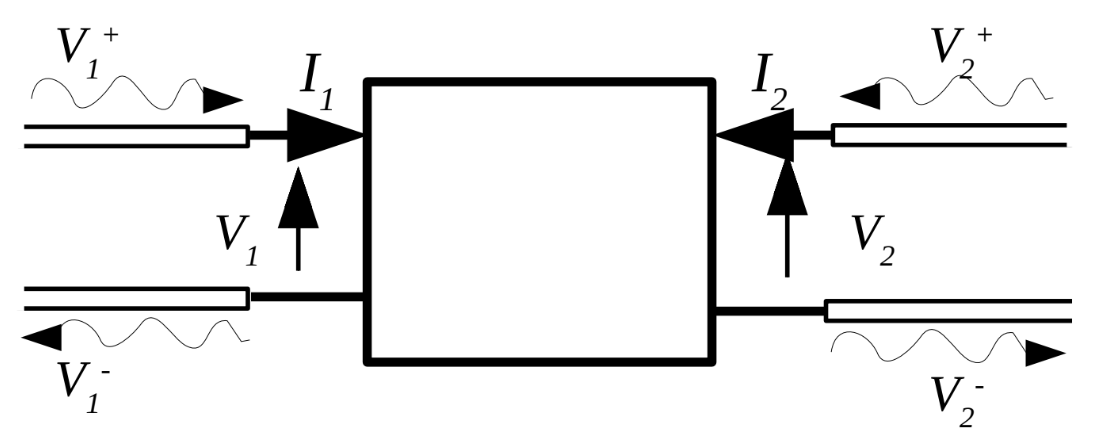
\includegraphics[width=.8\textwidth]{Images/figure38.png}
\end{center}
Scegliamo le \textbf{ampiezze delle onde incidenti} come \textbf{variabili indipendenti}:
\begin{squared}[violet]
    \begin{dcases}
    V_1^- = S_{11} V_1^+ + S_{12} V_2^+\\
    V_2^- = S_{21} V_1^+ + S_{22} V_2^+
    \end{dcases}
    \implies \underline{V}^- = \underline{\underline{S}} \underline{V}^+
\end{squared}
I coefficienti $S_{i,j}$ sono \textbf{adimensionali} e detti \textbf{parametri di Scattering}.
\section{Reciprocità}
Dividiamo due casi:
\begin{center}
    \textbf{(a)}\\
    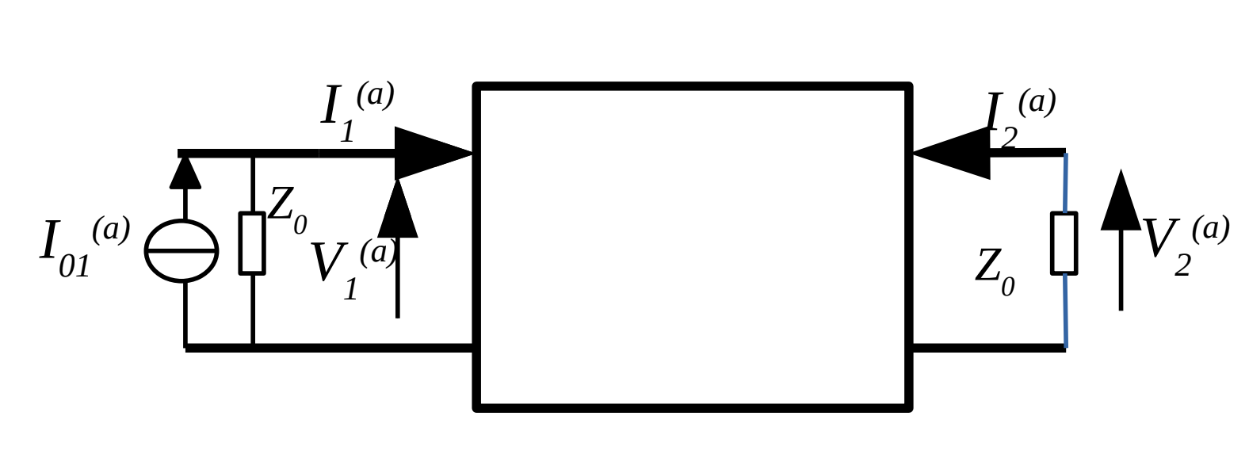
\includegraphics[width=.7\textwidth]{Images/figure39.png}
\end{center}
\begin{equation*}
    I_{01}^a = 2 I_1^a = 2 \frac{V_1^{a+}}{Z_0}
\end{equation*}
\begin{center}
    \textbf{(b)}\\
    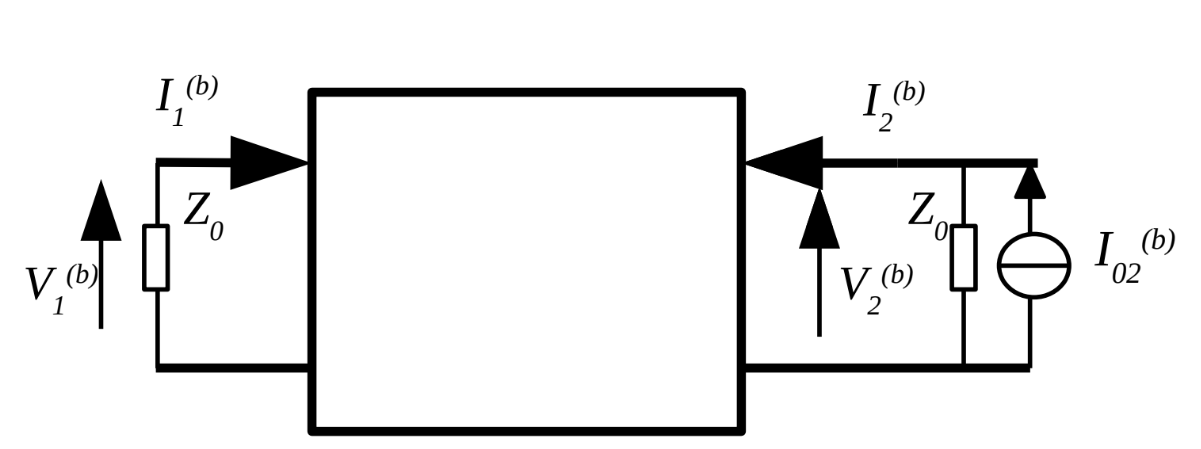
\includegraphics[width=.7\textwidth]{Images/figure40.png}
\end{center}
\begin{equation*}
    I_{02}^b = 2 I_1^b = 2 \frac{V_2^{b+}}{Z_0}
\end{equation*}
Il \textbf{teorema di reciprocità} applicato in questo caso ci da:
\begin{equation*}
    I_{01}^a V_1^b = I_{02}^b V_2^a
\end{equation*}
Che sostituendo le \textbf{correnti} diventa:
\begin{equation*}
\tag{x}
    V_1^{a+} V_1^b =V_2^{b+} V_2^a
\end{equation*}
Calcoliamo $ V_2^a$:
\begin{equation*}
     V_2^a = \cancel{V_2^{a+}} + V_2^{a-} = V_2^{a-} = S_{21} V_1^{a+} + \cancel{S_{22} V_2^{a+}}
\end{equation*}
\begin{equation*}
    \implies V_2^a = S_{21} V_1^{a+}
\end{equation*}
Calcoliamo $ V_1^b$:
\begin{equation*}
     V_1^b = \cancel{V_1^{b+}} + V_1^{b-} = V_1^{b-} = \cancel{S_{12} V_1^{b+}} + S_{12} V_2^{b+}
\end{equation*}
\begin{equation*}
    \implies V_1^b = S_{12} V_2^{b+}
\end{equation*}
Sostituiamo in (x):
\begin{equation*}
     \cancel{V_1^{a+}} S_{12} \cancel{V_2^{b+}} = \cancel{V_2^{b+}} S_{21} \cancel{V_1^{a+}}
\end{equation*}
\begin{squared}
    \implies S_{12} = S_{21} \implies \underline{\underline{S}} = \underline{\underline{S}}^T
\end{squared}

\section{Senza Perdite}
\textbf{Assenza di perdite} vuol dire che la \textbf{somma delle potenze attive alle due porte è nulla}.\\
Possiamo calcolare la potenza alle due porte tramite la \textbf{differenza della potenza incidente e quella riflessa}, quindi:
\begin{equation*}
    P_{diss} = \frac{1}{2} \frac{|V_1^+|^2}{Z_0} - \frac{1}{2} \frac{|V_1^-|^2}{Z_0} + \frac{1}{2} \frac{|V_2^+|^2}{Z_0} - \frac{1}{2} \frac{|V_2^-|^2}{Z_0} = 0
\end{equation*}
\begin{equation*}
    \implies \cancel{\frac{1}{2}} \frac{|V_1^+|^2}{\cancel{Z_0}} + \cancel{\frac{1}{2}} \frac{|V_2^+|^2}{\cancel{Z_0}} = \cancel{\frac{1}{2}} \frac{|V_1^-|^2}{\cancel{Z_0}} + \cancel{\frac{1}{2}} \frac{|V_2^-|^2}{\cancel{Z_0}}
\end{equation*}
\begin{equation*}
    \implies |V_1^+|^2 + |V_2^+|^2 = |V_1^-|^2 + |V_2^-|^2
\end{equation*}
In \textbf{forma matriciale} sarebbe:
\begin{equation*}
    \begin{bmatrix}
    V_1^{+^*}, V_2^{+^*}
    \end{bmatrix}
    \begin{bmatrix}
    V_1^{+}\\ V_2^{+}
    \end{bmatrix}
    =
    \begin{bmatrix}
    V_1^{-^*}, V_2^{-^*}
    \end{bmatrix}
    \begin{bmatrix}
    V_1^{-}\\ V_2^{-}
    \end{bmatrix}
\end{equation*}
\begin{equation*}
    {\underline{V}}^{+^H} {\underline{V}}^+ = {\underline{V}}^{-^H} {\underline{V}}^-
\end{equation*}
\begin{equation*}
    {\underline{V}}^{+^H} {\underline{V}}^+ = \left(\underline{\underline{S}}{\underline{V}}^{+} \right)^H \left(\underline{\underline{S}}{\underline{V}}^{+} \right)
\end{equation*}
\begin{equation*}
    \implies \underline{{V}}^{+^H} {\underline{V}}^{+} = {\underline{V}}^{+^H} \left(\underline{\underline{S}}^H\underline{\underline{S}}\right){\underline{V}}^{+}
\end{equation*}
Dato che deve valere che $\forall  \ \underline{V}^{+}  $
\begin{equation*}
    \implies \underline{\underline{S}}^H\underline{\underline{S}} = \underline{\underline{I}}
\end{equation*}
Analizziamo ora elemento per elemento $\underline{\underline{S}}$ per \textbf{verificare se rispetta la condizione}:
\begin{equation*}
    \begin{bmatrix}
   S_{11}^* & S_{12}^* \\
   S_{21}^* & S_{22}^*
    \end{bmatrix}
    \cdot 
    \begin{bmatrix}
   S_{11} & S_{12} \\
   S_{21} & S_{22}
    \end{bmatrix}
    =
    \begin{bmatrix}
   1 & 0 \\
   0 & 1
    \end{bmatrix}
\end{equation*}
Quindi:
\begin{equation*}
    \begin{dcases}
    |S_{11}|^2 + |S_{12}|^2 = 1 \\
    S_{12}^*S_{11} + S_{22}^* S_{12} = 0\\
    S_{11}^*S_{12} + S_{12}^* S_{22} = 0\\
    |S_{12}|^2 + |S_{22}|^2 = 1
    \end{dcases}
\end{equation*}
Ricordando che $S_{12} = S_{21}$:
\begin{equation*}
    |S_{22}|^2 = 1 - |S_{12}|^2 ,\quad |S_{21}|^2 = 1 -  |S_{22}|^2 \implies |S_{22}|^2 = |S_{11}|^2 = s^2
\end{equation*}
Da cui:
\begin{squared}
\begin{dcases}
    S_{11} = s e^{j \varphi_{11}}\\
    S_{22} = s e^{j \varphi_{22}}\\
    S_{12} = S_{21} = \sqrt{1 - s^2} e^{j \varphi_{12}}
\end{dcases}
\end{squared}
Sostituiamo in $S_{11}^*S_{12} + S_{21}^* S_{22} = 0$:
\begin{equation*}
    s e^{-j \varphi_{11}} \sqrt{1 - s^2} e^{-j \varphi_{12}} + \sqrt{1 - s^2} e^{-j \varphi_{12}} s e^{-j\varphi_{22}} = 0
\end{equation*}
Da cui:
\begin{equation*}
    e^{-j \varphi_{11}}e^{j \varphi_{12}}+e^{-j \varphi_{12}}e^{j \varphi_{22}} = 0
\end{equation*}
Ovvero:
\begin{equation*}
    \begin{aligned}
    &e^{j(\varphi_{12} - \varphi_{11})} = -e^{j(\varphi_{22}-\varphi_{12})}\\
    &e^{j(\varphi_{12} - \varphi_{11})} = e^{j(\varphi_{22}-\varphi_{12} + \pi)}\\
    &\varphi_{12} - \varphi_{11} = \varphi_{22}+\varphi_{12} + \pi + 2n\pi\\
    &2\varphi_{12} = \varphi_{22}+\varphi_{11}+ \pi + 2n\pi
    \end{aligned}
\end{equation*}
\begin{squared}
    \varphi_{12} = \frac{\varphi_{22} + \varphi_{11}}{2}  \pm \frac{\pi}{2}
\end{squared}